\chapter{Simulation corrections}
\label{chap:simulation-corrections}

%\chapterquote{}{}

\section{Introduction}

This chapter details the corrections applied to the Monte Carlo (MC) simulated 
events aimed at improving the description of observed events (data) by the MC.
These corrections are typically understood in terms of a scale multiplied to a
quantity, also known as a scale-factor, hence one represents no deviation from
the nominal MC prediction. There are two main categories of corrections used
in this analysis. The first corresponds to changing the weighting of a MC
event, known as an event-based correction. The weight given to a MC event is
the product of the cross-section of the particular process and the integrated
luminosity, $\sigma \mathcal{L}$. The cross-section $\sigma$ is calculated to
the highest order available in both the strong and electroweak coupling
constants, whereas the luminosity $\mathcal{L}$ is measured by the \CMS and
surrounding detectors. Event-based corrections will scale this weight on an
event-by-event basis, however, the sum of the weights over all events should
remain unchanged. The second set of corrections represents a shift in an
parameter, such as altering the momentum of an object, hereby known as an
object-based correction. Typical aggregation of information is in the form of
histograms where data in a particular bin is determined from the total number
of events within the bin's criteria, whereas the MC contribution is a sum over
the weights for the same criteria. Therefore, the event-based corrections
simplify to a scale up or down to an event's contribution in the sum. However,
object-based correction alter which bin the event may fall in. Both
corrections, even if unity, are associated with an uncertainty to alter the
correction up or down resulting in an alternative histogram under different
variation hypotheses. These hypotheses are used later in the statistical
interpretation of the results.

An event-based correction is determined by measuring the efficiency of a
selection or requirement in data, \effdata, and again in MC, \effmc,
parameterised in terms of observables $\vec{x}$ resulting in a scale-factor,
$\hat{f}$, of
%
\begin{equation}
    \hat{f}(\vec{x}) = \frac{\effdata(\vec{x})}{\effmc(\vec{x})}\ .
\end{equation}
%
This reweighting procedure attempts to have MC replicate the observed
efficiency for a particular selection. The efficiencies are measured with a
few different techniques, discussed in detail below.


\subsection{Tag and probe method}

A common technique to measure the efficiency in data is known and the tag and
probe method. This technique involves the selection of events containing two
candidates: a tag which must pass a tight set of restrictions $T$ to firmly
avoid misidentification, and a probe which passes very loose requirements $P$.
The events are such that the tag infers knowledge of the probe, for example,
in \IDYll where one lepton is a tag and the other a probe. The efficiency of a
selection $S$, given the probe requirements $P$, is determined by counting
events:
%
\begin{equation}
    \varepsilon(S|P) = \frac{N(S\cap T\cap P)}{N(T\cap P)}\ ,
\end{equation}
%
where $N(R)$ is the number of events passing some set of requirements $R$. For
a tag and probe from a \PZ boson decay the event counting is taken from the
signal by performing a maximum likelihood fit to the \PZ beak with a falling
background. A similar procedure can be performed in MC, however, knowledge of
the generator-level objects and process omits the need for a tag. Other
techniques in use are detailed in line.


\section{Trigger Efficiency}

The trigger selection discussed in Sec.~\ref{sec:baseline-selection} collect a
particular set of events for the analysis; however, limitations in the
reconstruction available to the \HWT and \SWT results in a loss of events. To
replicate the data collection in simulated events the efficiency of a trigger
selection is measured. The trigger selections are split into the muon,
electron and \ptmiss categories.


\subsection{Muon trigger efficiency}

The muon trigger efficiency \cite{CMS-DP-2017-056} is measured with the tag
and probe method where the tag selection $T$ and $P$ selection must pass the
full set of analysis requirements apart from the \pt and $\eta$ criteria for
the probe. This allows the parameterisation of the muon efficiency with \pt
and $\eta$ as the performance is expected to be highly dependent on these
variables. The tag is also required to cause the event to pass the muon
trigger selection such that the event is stored. The events are subsequently
split into all probes and those passing the muon triggers with further
division into independent \pt and $\eta$ bins. In each category the maximum
likelihood fit is performed to the invariant mass of the two muons to extract
the signal, modelled as a Breit-Wigner convoluted by a gaussian distribution,
and background, modelled as a falling exponential, contributions in each bin.
The efficiency is determined in each bin from the ratio of signal events where
the probe passes the muon trigger selection to signal events without this
requirement. The statistical uncertainty on the signal events is propagated
through to the efficiencies with additional systematic uncertainties by
performing the fit varying, in turn, the number of invariant mass bins,
invariant mass range, signal and background models, tag selection and probe
multiplicity. During the 2016 data-taking period, saturation issues in the
pre-amplifier chips for the tracker resulted in a loss of hits. This effect
was mitigated in the later part of this period and further reduced by a
re-processing of the data. Nevertheless, the muon trigger efficiencies are
split into the initial part and final part of the data-taking period, as shown
in Fig.~\ref{fig:muon-trigger-efficiency}.

\begin{figure}[htbp]
    \centering
    \begin{subfigure}[b]{0.49\textwidth}
        \centering
        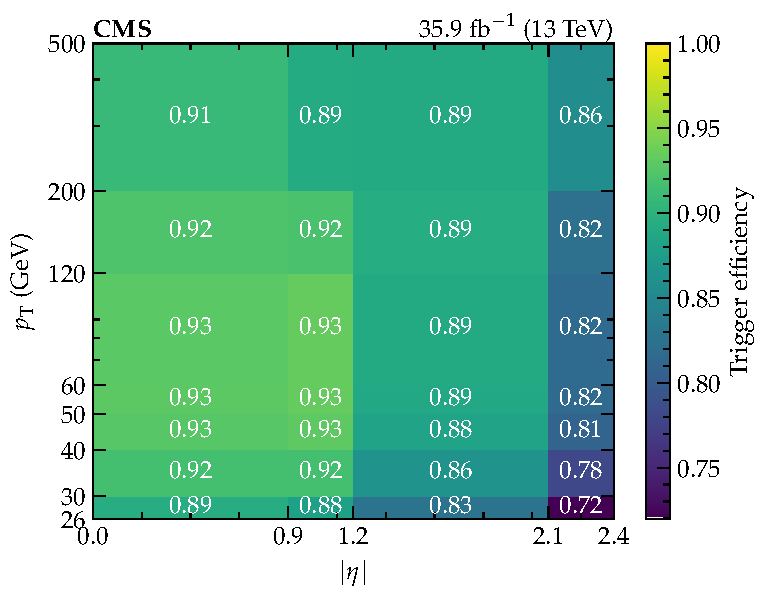
\includegraphics{chapters/041_corrections/images/efficiencies/triggers/muons/muon_RunBCDEF_trigger_efficiency.pdf}
        \caption{Initial data-taking period}
        \label{subfiga:muon-trigger-efficiency}
    \end{subfigure}
    \hfill
    \begin{subfigure}[b]{0.49\textwidth}
        \centering
        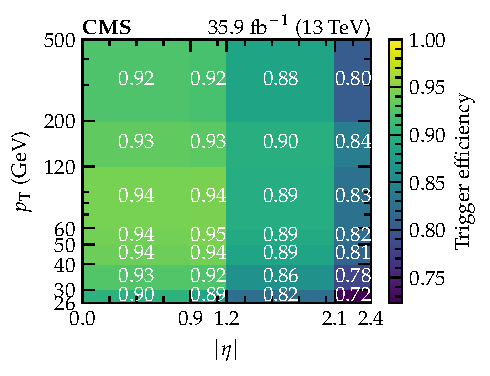
\includegraphics{chapters/041_corrections/images/efficiencies/triggers/muons/muon_RunGH_trigger_efficiency.pdf}
        \caption{Final data-taking period}
        \label{subfigb:muon-trigger-efficiency}
    \end{subfigure}
    \caption{
        Muon trigger efficiencies parameterised by its \pt and \aeta, split by
        the data-taking period. The trigger efficiency is lower in the endcaps
        where the muon background rate is larger and for low \pt muons where
        the track reconstruction is poorer. Inefficiencies for high \pt muons
        result from mitigating misidentified charged hadrons or issues in
        reconstructing the \pt for straight tracks. Most of the trigger
        efficiency arises from the \HWT decision which is heavily constrained
        by the timing budget. The differences between the data-taking periods
        are at most $2\%$, with significant overlap within the uncertainties.
    }
    \label{fig:muon-trigger-efficiency}
\end{figure}

This efficiency, $\varepsilon_i$, is associated to a single muon; however,
events collect with higher muon multiplicities were triggered by any of the
muons, hence the efficiency associated with the event, $\varepsilon$, for any
number of muons is
%
\begin{equation}\label{eq:electron-event-trigger-efficiency}
    \varepsilon = 1 - \prod_{i\in\mathrm{muons}} ( 1 - \varepsilon_i )\ ,
\end{equation}
%
as follows from a binominal distribution where at least one muon must pass the
trigger selection. This efficiency scales the MC event weight in regions
collected by the muon triggers with a luminosity-weighted average of the
initial and final data-taking periods.


\subsection{Electron trigger efficiency}

The electron trigger efficiency measurement \cite{CMS-DP-2017-004} follows a
similar procedure to the muons with a tag selection aligned with the analysis
and a probe with relaxed kinematic criteria. The pair of electrons are formed
into a \PZ boson candidate with a fit to the invariant mass distribution to
extract the signal contribution and determine the efficiency of the electron
trigger selection. Systematic uncertainties are determined with the same
method detailed for the muon trigger efficiencies. The efficiencies for the
electron trigger selection is shown in
Fig.~\ref{fig:electron-trigger-efficiency} and follow the same event-based
efficiency in Eq.~\ref{eq:electron-event-trigger-efficiency}.

\begin{figure}[htbp]
    \centering
    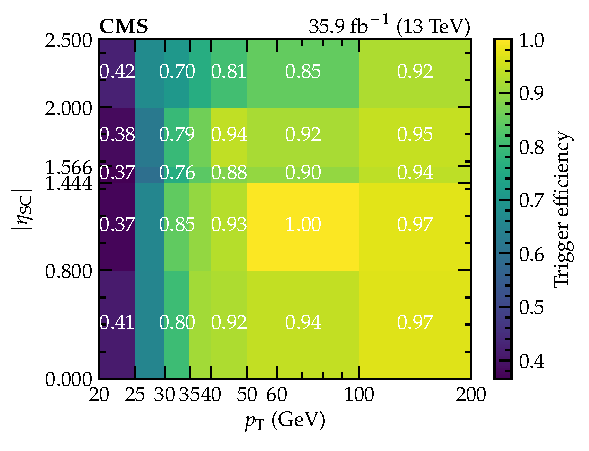
\includegraphics{chapters/041_corrections/images/efficiencies/triggers/electrons/electron_trigger_efficiency.pdf}
    \caption{
        Electron trigger efficiency with a threshold of ${\pt>\SI{27}{GeV}}$, parameterised with the \pt and absolute supercluster position in $\eta$, $|\eta_{\mathrm{SC}}|$. The low \pt inefficiency is driven by the trigger threshold and the efficiency in the partially uninstrumented gap in the \ECAL is shown in the bin ${1.444<|\eta_{\mathrm{SC}}|<1.566}$.
    }
    \label{fig:electron-trigger-efficiency}
\end{figure}


\subsection{\ptmiss trigger efficiency}

\begin{itemize}
    \item Here we go.
    \item Need to revisit this
\end{itemize}



\section{Object-based corrections}


Corrections based on the physics objects of an event may alter the weight of
the event and will be discussed here, along with corrections to particle
kinematics. Furthermore, the selection discussed in
Sec.~\ref{sec:categorisation} are not strict requirements on MC events. In
particular, events with an object and an associated scale-factor $f$ will
contribute to the object selection regions by a weight $f$, however, this
event will also contribute to object veto regions by a weight $1-f$ such that
the total contribution of the event across all regions becomes $1$, leaving
the overall cross-section unchanged. When $f=1$ the strict veto requirements
are recovered and the event does not enter the object vetoing regions. The
uncertainty on the efficiency of a selection is encoded in the scale-factor,
$\delta f$, such that the weight where the event is vetoed is
%
\begin{equation}
    1 - f = 1 - \mathcal{N}_f(f_0,\delta f_1) = 1 - (f_0 + \mathcal{N}_f(0,1)\delta f_1)\ ,
\end{equation}
%
where $f_0$ is the central value of the scale-factor, $\delta f_1$ is its
$1\sigma$ variation and $\mathcal{N}_f(\mu,\sigma)$ is a gaussian distributed
random variable with a mean $\mu$ and width $\sigma$. Therefore, MC events
vetoed may still contribute to a region, albeit weighted down or possibly
negatively. Such a procedure is performed with muons, electrons, photons,
\Ptauh-leptons abd b-tagged jets for both the veto and selection definitions.


\subsection{Muons}

Muons are formed from tracks with identification and isolation requirements to
reduce misidentification. The efficiency in selecting muons is factorised into
%
\begin{equation}
    \varepsilon_{\mu} = \varepsilon_{\mu}(\mathrm{ID}|\mathrm{track}) \varepsilon_{\mu}(\mathrm{Iso}|\mathrm{ID})\ ,
\end{equation}
%
where the track collection efficiency is near $100\%$ and hence omitted. The
parameter $\varepsilon(\mathrm{ID}|\mathrm{track})$ is the identification
efficiency for a given set of tracks and
$\varepsilon(\mathrm{Iso}|\mathrm{ID})$ is the isolation efficiency given a
collection of muons passing identification requirements. Since the analysis
uses two muon identification and isolation requirements the efficiency must be
measured for both the veto and selection criteria. The measurement is
performed using the tag and probe technique with the tag passing a tight set
of requirements ensuring minimal misidentifications and a set of tracks as a
probe or muons with an isolation requirement. Similarly to the muon trigger
efficiency, the events are collected into bins of \pt and $\eta$ with a fit to
the invariant mass of the muon pair to extract the signal contribution for all
probes and probes passing the identification or isolation requirements,
allowing the efficiency to be determined. A similar approach is performed in
MC, however, the distinction of signal events is known, bypassing the need for
a fit allowing for the simple counting of events.

During the 2016 data-taking period, saturation issues in the pre-amplifier
chips for the tracker resulted in a loss of hits. This effect was mitigated in
the later part of this period and further reduced by a re-processing of the
data. Nevertheless, the identification and isolation efficiencies are split
into the initial part and final part of the data-taking period. The ratio of
the efficiencies measured in data and MC for each period is shown in
Fig.~\ref{fig:muon-id-iso-efficiency} and subsequently the product of the
identification and isolation scale-factors is applied as a correction to MC.

\begin{figure}[htbp]
    \centering
    \begin{subfigure}[b]{0.49\textwidth}
        \centering
        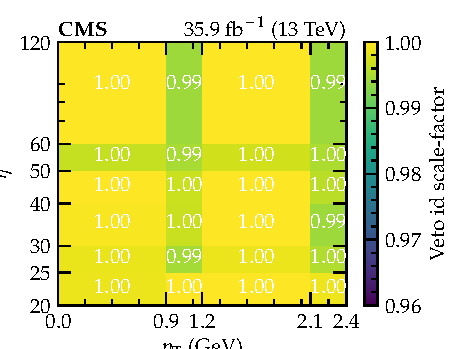
\includegraphics{chapters/041_corrections/images/efficiencies/objects/muons/muon_id_loose_runbf.pdf}
        \caption{Initial data-taking period}
        \label{subfiga:muon-id-scale-factors}
    \end{subfigure}
    \begin{subfigure}[b]{0.49\textwidth}
        \centering
        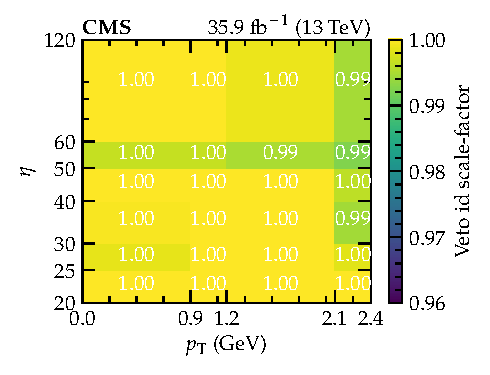
\includegraphics{chapters/041_corrections/images/efficiencies/objects/muons/muon_id_loose_rungh.pdf}
        \caption{Final data-taking period}
        \label{subfigb:muon-id-scale-factors}
    \end{subfigure}
    \begin{subfigure}[b]{0.49\textwidth}
        \centering
        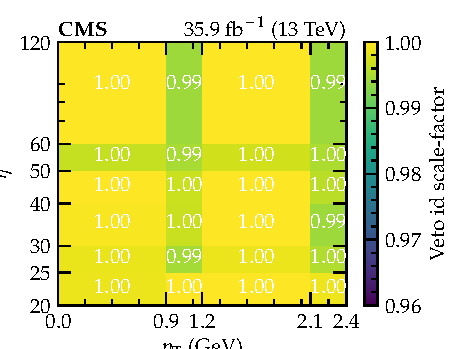
\includegraphics{chapters/041_corrections/images/efficiencies/objects/muons/muon_id_loose_runbf.pdf}
        \caption{Initial data-taking period}
        \label{subfiga:muon-id-scale-factors}
    \end{subfigure}
    \begin{subfigure}[b]{0.49\textwidth}
        \centering
        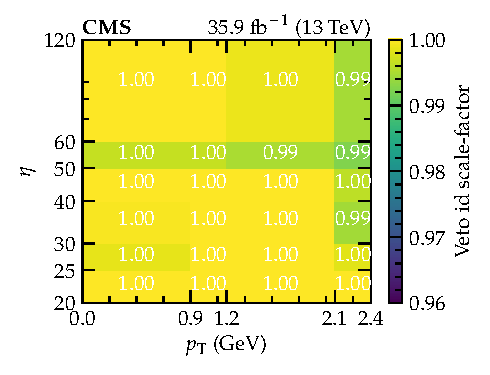
\includegraphics{chapters/041_corrections/images/efficiencies/objects/muons/muon_id_loose_rungh.pdf}
        \caption{Final data-taking period}
        \label{subfigb:muon-id-scale-factors}
    \end{subfigure}
    \includegraphics{}
    \caption{Caption}
    \label{fig:muon-id-scale-factors}
\end{figure}


\subsection{Electrons and Photons}

The efficiency of the identification and isolation of electromagnetic showers
are measured with the tag and probe technique in a similar manner to the
muon-based efficiencies. A fit to the invariant mass distribution of electron
pairs is performed to extract the signal yield in various probe \pt and $\eta$
bins. This allows the efficiencies to be determined with analogous
measurements in MC with the counting method. Systematic uncertainties are
determined from the variation in efficiencies from altering the tag selection,
signal model (template from MC or fully parameteric), background model, MC
generator (LO against NLO), and additional sources for the photon
identification efficiency to account for differences in the electron and
photon showers. The ratio of the efficiency in data and MC is determined,
shown in Fig.~\ref{fig:egamma-id-iso-efficiency} and applied as a correction
to MC.

\begin{figure}[htbp]
    \centering
    \includegraphics{}
    \caption{Caption}
    \label{fig:egamma-id-iso-efficiency}
\end{figure}

In addition, the efficiency for the reconstruction of GSF tracks matched to
\ECAL deposits is measured with the same method and shown in
Fig.~\ref{fig:electron-reco-efficiency}. Similarly, the efficiency from
vetoing photons with a consistent GSF track is measured with a similar method
in \IDYmmg, where the tag consists of a muon pair and the probe a
final state radiated photon. The ratio of the efficiency in data and MC for
the GSF track veto is shown in Fig.~\ref{fig:photon-trackveto-efficiency}.

\begin{figure}[htbp]
    \centering
    \includegraphics{}
    \caption{Caption}
    \label{fig:electron-reco-efficiency}
\end{figure}

\begin{figure}[htbp]
    \centering
    \includegraphics{}
    \caption{Caption}
    \label{fig:photon-trackveto-efficiency}
\end{figure}

Finally, the difference in the scale and resolution of electrons and photons
in data and MC is measured from the impact on the mean and width of the
invariant mass distribution in \IDYee events. A fit to the \PZ lineshape is
performed to extract the mean and width in data and MC. The observed
difference is used as a correction to electron and photon energies with
associated systematic uncertainties from the signal and background models, MC
generator and differences between the electron and photon showers.

% TODO: give a reference or attach the associated result?


\subsection{Jets}

The detector response to objects, especially the cluster of particles in jets,
is not linear. Therefore, a set of jet energy corrections are measured and
applied to map the reconstructed jet energy to the particle-level equivalent
(the energy of all generated particles originating from the parton excluding
neutrinos). A factorised approach is implemented with each level accounting
for different effects \cite{Khachatryan:2016kdb}.

The first step mitigates the contribution of particles from pileup vertices
which fall within the cone of the jet. This contribution is determined with
the random cone method in zero bias events and in simulations without any hard
interactions. Zero bias events are collected by randomly selecting collisions
regardless of their content. Since the hard interaction cross-section is small
this typically selected events with pileup interactions. The random cone
method consists of placing a random set of jet cones in a zero bias event,
clustering the particles falling within these cones, and determining the
energies of these jets. This energy represents the contribution to a jet from
pileup and is parameterised by the event energy density and jet \pt and
$\eta$. A systematic uncertainty is determined by comparing the correction
from the random cone method to the generator-level in MC.

The second step involves the correction to particle-level jets. Again, this is
determined from QCD dijet simulations by comparing the reconstructed jet \pt
to particle-level \pt, parameterised by the jet \pt and $\eta$. A systematic
uncertainty is determined for this correction as a result of its dependence on
the underlying detector calibrations with results from test beam studies.

The third and final step attempts to resolve residual differences between data
and MC. These corrections are applied to data since the aim is to replicate
the particle-level description which is only available in simulation. This
step is split into two stages: the first is an $\eta$-dependent correction
determined from dijet events with barrel jets used as a reference, and a
second a \pt-dependent scale difference between data and MC determined from
\IDYllj, \Igj and QCD multijet events. In these processes the jet energy
response is studied by comparing reconstructed jets to particle-level jets on
a jet-by-jet basis and also the whole hadronic activity from the correlation
of a particle-level jet to the missing transverse energy of the event. These
methods do not fully capture the dependence as a result of the correlation
between initial (ISR) or final state radiated (FSR) jets, therefore, an
additional correction is determined by probing the $\eta$-dependent
corrections with a selection to enhance the effect of this correlation. Along
with these corrections are associated systematic uncertainties to cover the
modelling in MC from an alternative event generator, statistical uncertainties
in the data due to trigger prescales, dependence of the corrections over the
data taking period, constituent particle energy uncertainties, and the
residual difference between the dijet, \Igj and \IDYllj samples after all
corrections have been applied.

In addition to the jet energy response difference between data and MC the
resolution is corrected for by comparing the balance of jets in a dijet event.
The scale determined to correct the MC resolution of the dijet balance is
applied to MC jets by smearing their energies with a random variable sampled
from a gaussian distribution with a scaled width. Systematic uncertainties
are determined by comparing the results to the particle-level imbalance, the
effect of removing particles below $\SI{10}{GeV}$, non-gaussian tails in the
resolution due to rare detector effects and the \pt-dependence is propagated
through the smearing.

All these corrections, and uncertainties, are propagated through all
jet-related quantities such as the missing transverse momentum where the jet
energy correction $k_i$, encoding both scale and resolution corrections,
results in a shift in the \ptmiss according to
%
\begin{equation}
    \vecptmiss \mapsto \vecptmiss + \sum_{i\in\mathrm{jets}}\vec{p}_{\mathrm{T},i} \left( 1 - k_i \right)\ ,
\end{equation}
%
where the sum is over clustered jets, i.e. ${\pt>\SI{15}{GeV}}$. 


\subsubsection{\Ptauh-tagged jets}

The jet energy corrections discussed are determined under the assumption the
jet originates from a parton. Therefore, the corrections are not applied to
\Ptauh-tagged jets, instead a scale-factor is determined to correct the
efficiency of \Ptauh-lepton identification in MC. The efficiency in data is
measured using the tag and probe method in \IDYtt decays, where one
$\tau$-lepton decays into a well reconstructed muon to tag the event and the
other into one of the hadronic decay modes to probe the identification. A fit
is performed to the invariant mass of the visible particles to extract the
signal contribution with templates taken from MC for the signal and most
backgrounds. Systematic uncertainties on the identification efficiency are
determined from the background normalisation, \ptmiss uncertainties and
limited sample sizes \cite{Sirunyan:2018pgf}.


\subsubsection{$b$-tagged jets}

Jets tagged as originating from $b$-hadrons have the jet energy corrections
applied, however, the $b$-tagging discriminant is not perfectly modelled in MC
due to detector simulation limitations and the accuracy of the generator
modelling the parton shower and hadronisation. Therefore, a scale-factor is
determined for the efficiency of $b$-tagging jets from QCD multijet,
muon-enriched jet, dilepton \Itt and single lepton \Itt samples
\cite{Sirunyan:2017ezt}. The efficiency is parameterised by the jet flavour
(grouped in $b$, $c$ and $udsg$ flavours), \pt and $\eta$. In simulation the
tagging efficiency is calculated by matching jets to generated jets with a
particular hadron flavour. Meanwhile, the data efficiency is measured with a
pure sample with jets of a certain hadron flavour using a selection which does
not bias the jets with respect to the variables in the tagging algorithm.
Systematic uncertainties associated to the $b$-tag scale-factors are
determined by varying background normalisations, branching fractions of
hadronic decays within the PDG uncertainties, reweighting the distribution of
the number of tracks, jet energy scale uncertainties, electron and muon
efficiencies and theoretical uncertainties from the event generators. In the
context of this analysis, $b$-tagged jets are vetoed, therefore the event
weight becomes
%
\begin{equation}
    w \mapsto w \prod_{i\in\mathrm{b-jets}} (1 - f_i)\ ,
\end{equation}
%
where $f_i$ is the scale-factor associated with the $i$-enumerated $b$-tagged
jet.


\section{Luminosity}

The integrated luminosity $\mathcal{L}$ measured for the data-taking period
directly scales the weight of a MC event. At \CMS the pixels, drift tubes, HF
and other detectors perform complimentary measurements of the luminosity by
rate counting, $R$, for visible processes with a cross-section
$\sigma_{\mathrm{vis}}$. The luminsoity is determined as
%
\begin{equation}
    \mathcal{L} = \frac{R}{\sigma_{\mathrm{vis}}}\ ,
\end{equation}
%
where the visible cross-section and calibrations of each detector is performed
by conducting Van der Meer scans \cite{vanderMeer:296752} prior to data-taking
collisions. The data collected during 2016 corresponds to an integrated
luminosity of ${\SI{35.9}{fb^{-1}}}$ with uncertainties from the precision of
the visible cross-section and calibration measurements along with
extrapolations to data-taking collisions resulting in a $2.5\%$ uncertainty
\cite{CMS:2017sdi} on the luminosity measurement.


\section{Pileup reweighting}

The pileup overlay applied to each simulated event is generated by the \PYTHIA
package with the number of pileup vertices sampled from a poisson distribution
with a tail to higher vertex multiplicities. In data, for a given
instantaneous luminosity, the number of pileup vertices is expected to be
poisson distributed. Therefore, a reweighting procedure corrects the MC
distribution to reflect that observed in data, without altering the
normalisation determined from the product of the process cross-section and the
integrated luminosity. The number of interactions in data is estimated from
the measured luminosity in each bunch crossing and the average total inelastic
cross-section. Furthermore, data measurements are averaged over periods of
constant instantaneous luminosity to compare with the mean of poisson
distribution sampled in MC, rather than the number of vertices in a particular
event. The total inelastic cross-section is measured by \CMS to be
${\SI{69.2}{mb}}$ with an uncertainty of $4.6\%$ for the nominal and
variational templates for the reweighting procedure used in the statistical
interpretation of the results. The magnitude of the reweighting and these
uncertainty bands are shown in Fig.~\ref{fig:pu-reweighting}.

\begin{figure}[htbp]
    \centering
    \includegraphics{}
    \caption{Caption}
    \label{fig:pu-reweighting}
\end{figure}


\section{\ECAL timing degradation}

A gradual degradation in the \ECAL timing has caused some \HWT \ECAL towers to
be associated with the incorrect bunch crossing (BX). The \HWT logic prevents
three successive bunch crossings to be accepted to avoid buffer overflows.
Therefore, the deposit in the \ECAL is wrongly associated to an early crossing
which may lead to a \HWT accept, later discarded in the \SWT where the timing
issue is not present. However, the correct crossing is vetoed by the \HWT
logic resulting in a loss in efficiency in the data collection. This primarily
affects events with \ECAL deposits in the endcaps where the timing degradation
is most prevalent. The efficiency of this issue is measured by collecting
immune events which occur three bunch crossings after a \HWT accepted
crossing. The immune event is labelled as $\mathrm{BX}+0$ and the
$n$-enumerated crossing before as $\mathrm{BX}-n$ and after as
$\mathrm{BX}+n$. Since $\mathrm{BX}-3$ is accepted by the \HWT the crossings
$\mathrm{BX}-2$ and $\mathrm{BX}-1$ are vetoed, hence they cannot veto
$\mathrm{BX}+0$. The event is tagged as affects by the timing degradation if
an \HWT object associated to $\mathrm{BX}-1$ or $\mathrm{BX}-2$ would have
vetoed the event. This allows the efficiency to be determined and
parameterised for jets and photons with their \pt and $\eta$. In MC the
efficiency of this issue is determined from a product over the measured
efficiencies associated to each object which is applied as a correction to the
event weight. Along with this, a systematic uncertainty is determined from
statistical uncertainty of the immune sample or a conservative $20\%$ on the
correction relative to $1$, whichever is largest.


\section{Theory corrections}

The cross-section applied directly to the event weight of a MC process is
calculated by theoretical predictions of the highest available order in the
strong and electroweak (EW) coupling constants. Associated systematic
uncertainties are determined by varying the QCD factorisation and
renormalisation scale up and down by a factor of two independently and fully
correlated for six variations with the largest variations taken as the
systematic uncertainty. In addition, the uncertainties from the measurements
of the sampled \NNPDF parton distribution functions (PDF) \cite{Ball:2014uwa}
are propagated by 100 variations, each randomly sampled from the original
distributions of the PDFs.

An alternative method is applied to the signal and dominant \IVj processes.
These are generated at NLO in the strong coupling constant, however, instead
of scaling the normalisation up to the highest order available a reweighting
of the boson \pt distribution is performed for a more accurate prediction.
This approach reweights the MC to NNLO QCD and NLO EW with next-to-leading
logarithms (NLL) EW corrections \cite{Lindert:2017olm}. This procedure scales
the cross-section parameterised by the boson \pt, determined from the
generated decay products (with photons within ${\Delta R<0.1}$ of charged
leptons summed into their 4-momentum). Systematic uncertainties determined for
the QCD corrections include variations in the factorisation and
renormalisation scales with the addition of a possible boson \pt dependence
and encoding the correlation between the \IZj and \IWj processes. Another set
of systematic uncertainties are determined for the EW corrections to cover
higher-order effects and an additional systematic uncertainty on unaccounted
contributions from diagrams of mixed order in the strong and EW coupling
constants by taking the difference between an additive and factorised
combination of the separate QCD and EW corrections. The PDF uncertainties are
propagated with the same procedure as for other generated processes. The full
set of uncertainties are detailed in Tab.~\ref{tab:qcdew-systematics}.

\begin{table}[htbp]
    \centering
    \begin{tabular}{lccp{9cm}}
        \hline \hline
        Label & \IVj & Other & Description \\
        \hline
        \uncqcdone & \checkmark & \checkmark & Factorisation and renormalisation scale variations. \\
        \uncqcdtwo & \checkmark & & Boson \pt dependence of the QCD scales. \\
        \uncqcdthr & \checkmark & & Correlations between QCD effects in \IZj and \IWj processes. \\
        \hline
        \uncewone & \checkmark & & Unknown Sudakov logarithms beyond NNLO. \\
        \uncewtwo & \checkmark & & $5\%$ of the absolute full NLO EW correction for a conservative estimate of non-Sudakov factors. \\
        \uncewthr & \checkmark & & Difference between a naive and rigorous NLL Sudakov approximation. \\
        \hline
        \uncqcdewmix & \checkmark & & Mixing terms with strong and EW coupling vertices. \\
        \hline
        \uncpdf & \checkmark & \checkmark & 100 PDF variations. \\
        \hline \hline
    \end{tabular}
    \caption{
        All systematic uncertainties included from the theory prediction of
        process cross-sections with a tick for which processes the uncertainty
        affects split into either \IVj or other processes. A brief description
        of each is given.
    }
    \label{tab:qcdew-systematics}
\end{table}


\section{Summary}